\documentclass[11pt, oneside]{article}   	% use "amsart" instead of "article" for AMSLaTeX format
\usepackage{geometry}                		% See geometry.pdf to learn the layout options. There are lots.
\geometry{a4paper}                   		% ... or a4paper or a5paper or ... 
%\geometry{landscape}                		% Activate for for rotated page geometry
%\usepackage[parfill]{parskip}    		% Activate to begin paragraphs with an empty line rather than an indent
\usepackage{graphicx}				% Use pdf, png, jpg, or eps§ with pdflatex; use eps in DVI mode
\usepackage{array}							% TeX will automatically convert eps --> pdf in pdflatex		
\usepackage{amssymb}

\title{Requirement Engineering Process in AMIDST}
\author{The handsome AMIDST guys et. al.}
\date{Latest version, \today}							% Activate to display a given date or no date

\begin{document}
\maketitle

\begin{abstract}
To be done later....
\end{abstract}

\section{Introduction}

It is widely accepted that there is a clear link between proper system requirement and project success xx and xx.  Also, there is clear link between failure to understand requirements and project failure xx and xx.  Although requirement engineering (RE) process is very important, the academic field is still seen as immature xx. There is agreement on that a definition of a requirement is related to \emph{what} a system can do and not \emph{how} it is done.  Moreover, the community acknowledge that requirements must be elicited, specified and validated.  However, the agreements seem to end there and little uniformity on terminology is reached xx. It is therefore a reasonable strategy to inspect the important aspects or constraints in a project before choosing a paradigm for conducting a RE process.

This report contains a description on how the RE process was conducted in the AMIDST project.  Prior to project start, the importance of RE was well acknowledged as can be seen from the assignment of 23 out of 310 person months to requirement analysis.  Several challenges were identified early and they are summarised table \reffi{tab:challenges}:

\begin{table}
\caption{Challenges in the AMIDST RE process}
\vspace{1ex}
\begin{tabular}{
>{\raggedright\hspace{0pt}}m{8mm}%
>{\raggedright\hspace{0pt}}p{120mm}}
\hline
& \tabularnewline
1 & Very few participants/stakeholders had wide experience with RE, which had to be taken into account in any communication on the topic. \tabularnewline
2 & The project is a consortium of 7 partners, 4 industrial and 3 universities, which are situated in 4 different countries.  This imposed a constraint on the communication channels. \tabularnewline
3 & The software is expected to be compatible with three different systems in three completely different domains, with three different companies. Transference of domain knowledge from the industrial partners to the academic partners is clearly a challenge. \tabularnewline
4 & The software itself is based on graphical probabilistic models, which is difficult to learn for the industrial partners.  \tabularnewline
5 & The goal of the software is reaching targets that are highly innovational. Defining a requirement is linked with the perception of which design pattern one wants to follow xx.  Since a requirement is understood to be clear and of no ambiguity, it is more difficult to define it, when there is unclearity in which design patterns to follow xx. \tabularnewline
6 & It was not clear if hardware needed to be taken into account before the analysis was conducted. \tabularnewline
& \tabularnewline
\hline
\end{tabular}
\label{tab:challenges}
\end{table}

To date there is no common definition of RE.  Some definitions focus on elicitation of requirements and therefore the interaction with the user, while other focus on the documentation or specification.  A definition that takes both focus into account is the IEEE standard:

\emph{
\begin{enumerate}
\item The process of studying user needs to arrive at a definition of system, hardware or software requirements.
\item The process of studying and refining system, hardware or software requirements.
\end{enumerate}
}
However, based on the challenges that was outlined above it is clear that also representational, social and cognitive aspects need to be taken into account in the definition and we found some comfort in the definition by xx

\emph{a systematic process of developing requirements through an iterative co-operative process of analysing the problem, documenting the resulting observations in a variety of representation formats and checking the accuracy of the understanding gained.}

It is also of important to give clarity on what definition of requirement that will be taken in this report.  The IEEE standard is 

\emph{
\begin{enumerate}
\item A condition or capability needed by a user to solve a problem or achieve an objective. 
\item A condition or capability that must be met or possessed by a system or system component to satisfy a contract, standard, specification or other formally imposed document. 
\item A documented representation of a condition or capability as in 1 or 2.
\end{enumerate}
}

This definition has a clear focus on the user, the system or the system component and also which contract, standard or specification is needed to be met.  This is particularly tractable in the AMIDST project where most contributors understand only parts of the project. Notice, that this definition does not allow for a requirement to be to some degree optional,.  This is needed to meet challenge 5 in \ref{tab:challenges} and as an extension we will refer to \emph{optional requirements} when this is needed. The use of the term optimal requirement will only be used, when the system is required to meet only a fraction of the optional requirements.

\section{The requirements engineering process in AMIDST}

The overall requirement engineering process will be carried out in an iterative fashion that is expected to involve a high level of cooperation and interaction between the partners. During this process the document for the requirements analysis will be gradually refined and expanded. In figure \ref{REprocess1} a description and an illustration of the RE process within AMIDST, which is divided into into the following phases:
\begin{enumerate}
 \item Preparation I.  This phase started with Work package 1 and the collection of data characteristics.  
 \item Elicitation. The distribution of the present document/template marks the initialization of this phase.  Its aim is to get an initial high-level description of the different use cases and their requirements. This information should be specified by the use case providers (in this case Daimler). Please, consider that the use-cases and requirements (which should be within the scope of AMIDST) are the ones that will be addressed in the project. Once the use case providers return the present document with the requested information, we expect to provide feedback on the submitted information in order to refine the information in collaboration with the use case provider. At the end of the elicitation phase, we aim to have a first coherent description of the requirements for each use case provider.
 \item Prioritization. In this phase the use case providers should complete an extended version of the document template used in the previous phase. This template will firstly be used to link each of the requirements to the relevant work packages and tasks in the AMIDST project. Moreover, the template will also allow the use case providers to provide a more fine grained prioritization of the relevant requirements for the AMIDST framework.  
 \item Validation. In the last phase we will collect the requirements of the three use-case providers to get the ?big picture?.  We will then discuss to what extent the requirements can be accommodated within the project. Revisions and negotiations of the detailed requirements may therefore be necessary.  
 \item Evaluation and Testing. In this phase, focus will be on the elicitation of the evaluation and testing procedures that are going to be used in the AMIDST project. This phase starts with the distribution of a new document template. Its aim is to obtain a high level description of the evaluation and testing methods that will be used to measure the performance of the AMIDST framework in relation to the use cases elicited in the previous phases.
\end{enumerate}

\begin{figure}
\centering
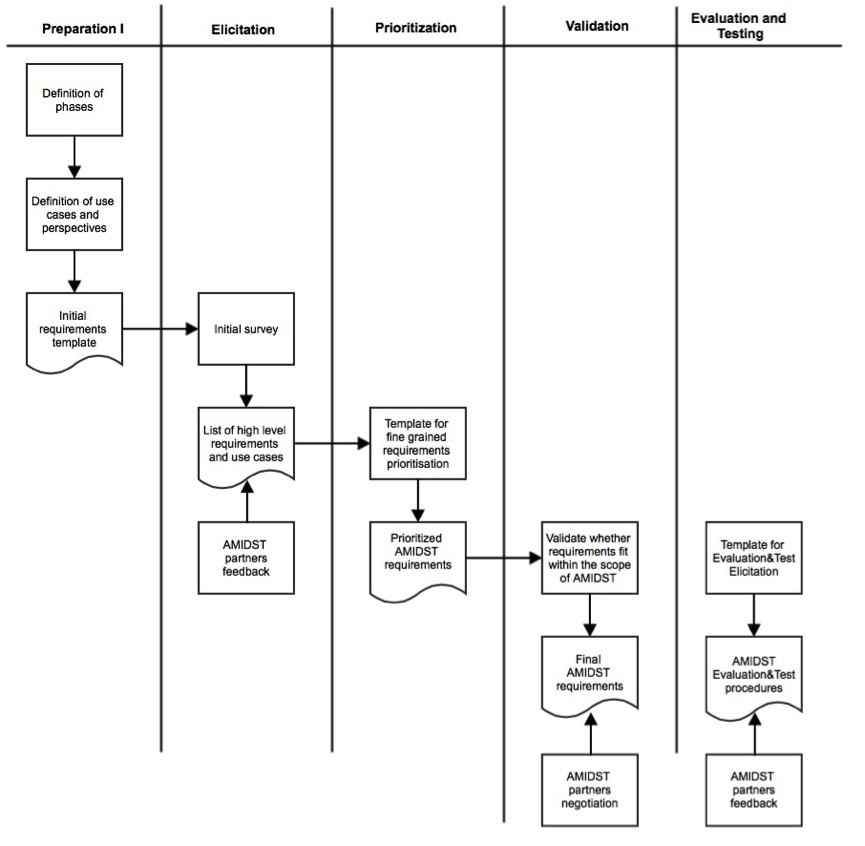
\includegraphics [keepaspectratio,width = 14cm] {REprocess1}
\caption{Description of the RE process in AMIDST.}
\label{REprocess1}
\end{figure}


\begin{figure}
\centering
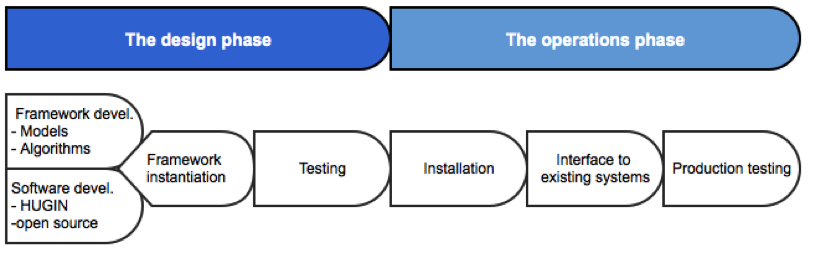
\includegraphics [keepaspectratio,width = 14cm] {REprocess2}
\caption{The table show key steps in the design and operation stages. Notice that each requirement can only be member of one step.}
\label{REprocess2}
\end{figure}

For the design stage we look for general functionality requirements for the system, i.e. what the system should do and support.  In the above figure, we detail key steps inside this phase. The first step consists of the design of the general framework (models and algorithms) as well as the design and development of the software tools. In a second step, the general framework and software will be instantiated for each specific use case. Finally, initial tests of the use case instantiated framework will be conducted.  
At this design phase, possible design requirements could e.g. address
\begin{itemize}
 \item the scope of the model
 \item the interpretability of the learned models
 \item the extent and type of domain knowledge that can be integrated into the models
 \item documentation
 \item etc. 
\end{itemize}
The requirements for the operation phase concern the functionality of the deployed system. In the above figure, we decompose this phase into three stages: installation, interface to existing systems, and production testing. The requirements for this phase could e.g. address
\begin{itemize}
 \item hardware constraints
 \item interfaces to existing software or data base systems
 \item inference functionality, i.e., what queries the system should be able to answer
\end{itemize}

\bibliographystyle{gNST}
\bibliography{ibr}


\end{document}  